\documentclass[10pt,conference]{IEEEtran}
\usepackage{graphicx}
\usepackage{listings}
\usepackage{color}

\lstset{
	basicstyle=\tiny,
	showstringspaces=false,
	%numbers=left,
	language=C,
	keywordstyle=\color{blue},
	frame=single
}

\begin{document}

\title{ADC Validation\\
	   for the Tiny6410 Board and the ARM 11 Processor}

\author
{
 \IEEEauthorblockN{Matthew Lopez}
 \IEEEauthorblockA{Electrical Engineering Department, College of Engineering \\
 San Jose State University, San Jose, CA 94303 \\ 
 E-mail: matthew.lopez@sjsu.edu}
}

\maketitle

%
% Abstract
%
\begin{abstract}
The purpose of this project is to validate that the ADC for the ARM11 processor works properly and to find the conversion for the input voltages. A Fast Fourier Transform is used to validate the ADC by looking at the power spectrum of the values. The ADC is determined to be working and a manual inspection of the values shows a linear relationship
\end{abstract}

%
% Introduction
%
\section{Introduction}
The goal of this project is two fold, 1) Validate the ADC for the ARM11 processor via the Fast Fourier Transform (FFT), and 2) Find the relationship between voltage and ADC values. A potentiometer is used to vary the voltage into the ADC. The voltage rages from 0 to 3.3VDC. The FFT is used, along with the computation of the power spectrum, to determine if the ADC is good. A manual reading of the voltages and ADC values as the potentiometer is varied is used to the determine the linear relationship between input voltage and ADC reported values. To accomplish this goal two software programs need to be written, the device driver and the user level program, and hardware needs to be acquired and built.

\subsection{Tiny6410 and ARM11 Hardware}
The ARM family of processors is a significant player in the processor space. Nearly 95 percent of smartphones, tablets, and other portable devices use an ARM processor \cite{ARMSales}. The Tiny6410 Development board uses the ARM11 processor manufactured by Samsung. The Tiny6410 board exposes the capabilities and I/O features of the ARM11 processor in a format that is easy to use, i.e. USB or Ethernet ports, as well as a touchscreen. An overview of the ARM11 processor and it's I/O can be found in figure \ref{ARM11BlockDiagram}.

\begin{figure}[ht!]
	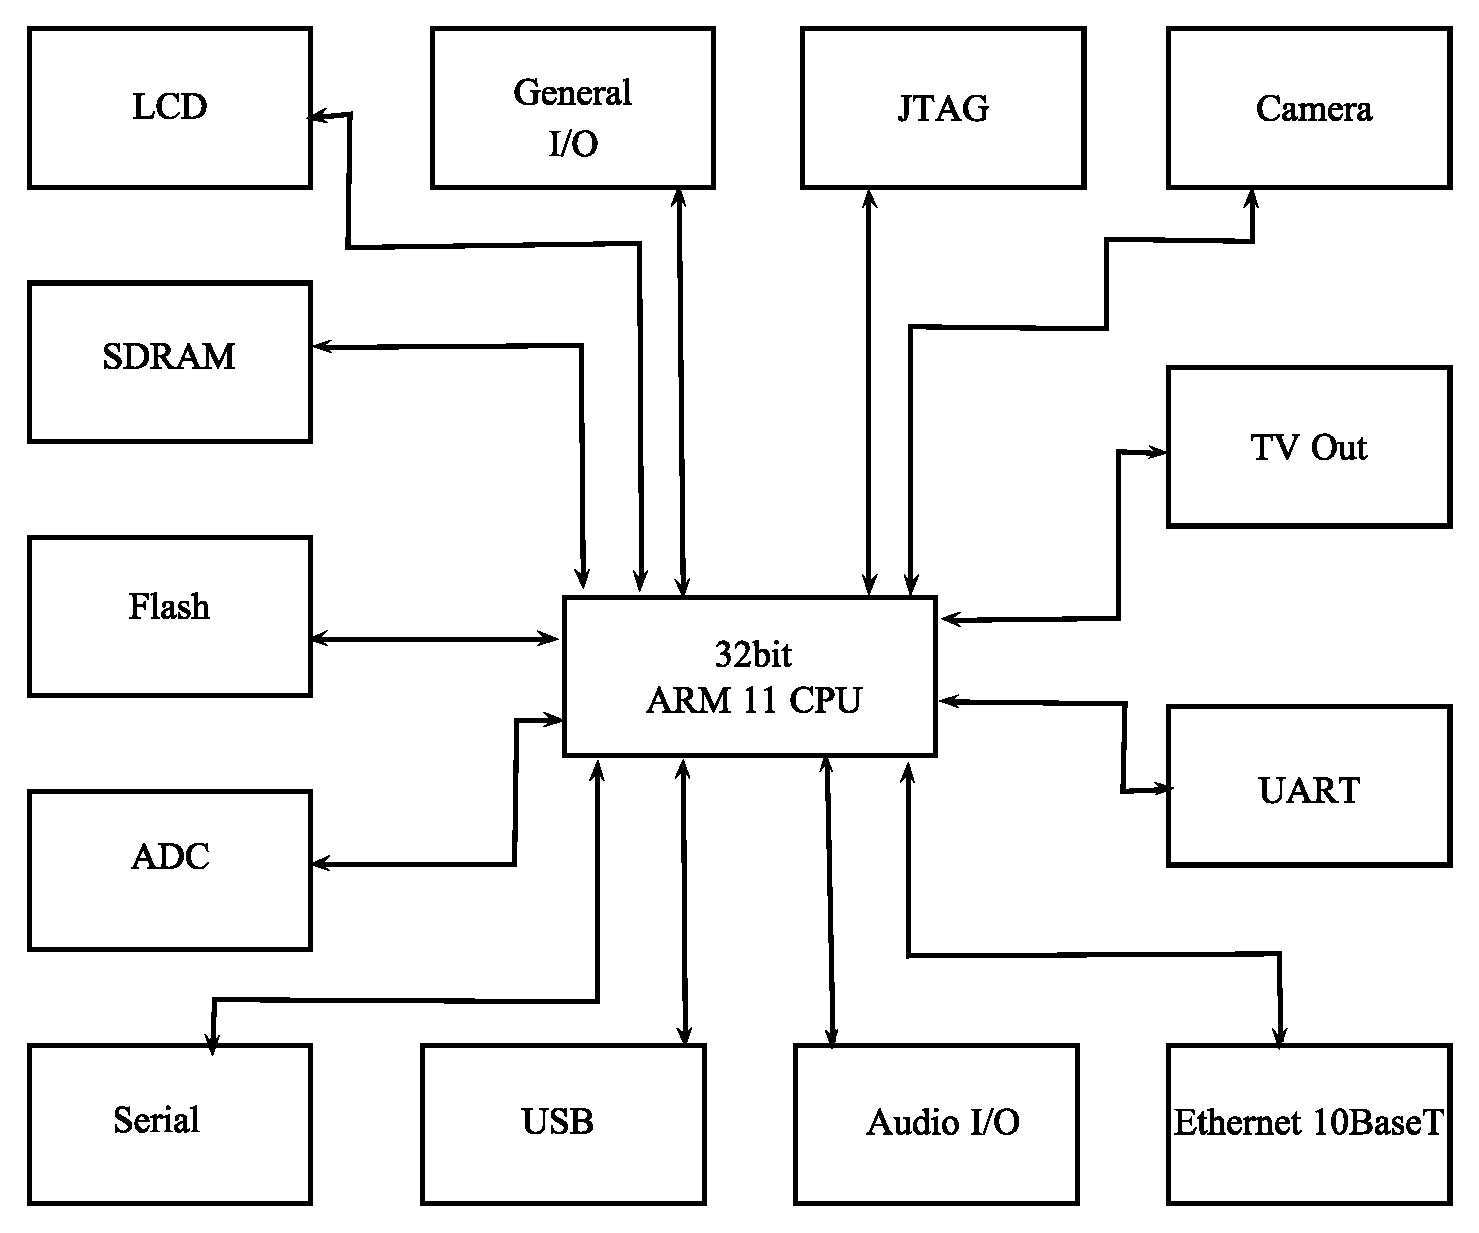
\includegraphics[scale=.30]{ARM11BlockDiagram}
	\caption{ARM11 and Tiny6410 I/O Block Diagram}\label{ARM11BlockDiagram}
\end{figure}



%
% Methodology
%
\section{Methodology}
This section will cover the objects and design of the hardware and the software.

\subsection{Objectives}
The objectives of the project are,
\begin{enumerate}
	\item Validate the ARM 11 ADC via the FFT and the power spectrum.
	\item Determine the linear relationship between input voltage and ADC values.
\end{enumerate}

\subsection{Hardware}
There are several components that make up the hardware used for this project.

\subsubsection{ARM11}\label{ARM11HW}
The ARM 11 processor provides 4 ADC channels with resolution of 10 or 12 bits. The channel selection, bit resolution, and other controls are done via the ADCCON control register \cite{Samsung}. The converted data from the analog device is placed into one of two data registers, ACDDAT0 or ADCDAT1 \cite{Samsung}.

The Tiny6410 board provides an interface to only 2 of the 4 ADC channels. On connector CON1, Channel 2 on pin AIN2 and Channel 3 on pin AIN3 \cite{HWHandout}.

\subsubsection{Prototype Board}\label{ProtoBoard}
The prototype board is a board that is separate from the Tiny6410 board. For this project the hardware on the prototype board consists of,
\begin{enumerate}
	\item Pins to connect the prototype board with the Tiny6410 board.
	\item Several resistors to limit the input voltage and current into the ADC.
	\item A potentiometer to adjust the voltage into the ADC and is used to help validate the ADC.
	\item A 5VDC power supply sourced from a USB port \cite{USB5VDC}.
\end{enumerate}

The resistors on the prototype board are used to limit the voltage to the ADC within the range of 0--3.3VDC. A simple voltage divider is used,
\begin{equation}\label{VoltageDivider}
	V_{adc} = \frac{R_2}{R_1 + R_2}V_{cc}
\end{equation}

\subsection{Software}\label{Software}
There are two software programs used for the project,
\begin{enumerate}
	\item The device driver.
	\item The user level program.
\end{enumerate}

\subsubsection{Device Driver}\label{DeviceDriver}
The device driver is the software that operates at the level of the Linux kernel and has direct access to the hardware. The device driver is broken up into several sections,
\begin{enumerate}
	\item Initialization. The control register is set to the default values. Pseudocode for the initialization can be found in listing \ref{SetADCCONCode}. The driver is also registered with the Linux kernel and can now be found by user level programs.
	\item Clean up. Deregister the driver from the Linux kernel.
	\item I/O Control. The driver needs to provide a method for user level programs to interact with the hardware. The device driver therefore implements the \emph{ioctl} function. The user level control function will send commands to the driver's \emph{ioctl} function to perform some action and the function will return a status or data value. The function can interact with the ADCCON register first mentioned in section \ref{ARM11HW} to modify the bit resolution and select which ADC channel to read from.
	\item Read. The device driver exposes a read function that allows the user level program to read from the ADC. The read function can interact directly from the hardware, reading from the ADCDAT register and then copying the data into a buffer in user space. A pseudocode implementation can be found at \ref{ReadADCDATCode}.
\end{enumerate}

\begin{lstlisting}[language=C, frame=single, caption=Pseudo Code to Prepare ADCCON,label=SetADCCONCode]
	// enable 10 bit resolution
	ADCCON |= (0<<16)
	// enable 12 bit resolution
	ADCCON |= (1<<16)
\end{lstlisting}

\begin{lstlisting}[language=C, frame=single, caption=Pseudo Code to read and write ADCDAT,label=ReadADCDATCode]
	// check if device ready
	// read data from device
	// copy the data into a user space buffer
	// return from function
\end{lstlisting}

\subsubsection{User Level Program}
The user level program is the software that operates at the level that the user has access to.  Direct access to the hardware is not allowed. As mentioned in the device driver section \ref{DeviceDriver}, the user level program uses \emph{ioctl} to interact with the device driver. The code is straightforward,
\begin{enumerate}
	\item The user invokes their request via a command line argument.  \emph{-r} to read the switch value. \emph{-l} followed by a zero or one to turn on or off the LED.
	\item The program translates the user into a command \emph{ioctl} from the device driver can understand. A common header file is shared between the user level program and the device driver to ensure the commands are consistent between the two programs.
	\item Call \emph{ioctl} with the appropriate command and read the results or error status.
\end{enumerate}
The pseudocode can be found in listing \ref{UserLevelProg}.

\begin{lstlisting}[language=C, frame=single, caption=User Level Pseudo Code,label=UserLevelProg]
	// read the user input and set the command
	if (input == '-b0')
		cmd = 10BIT_RESOLUTION
	else if (input == '-b2' )
		cmd = 12BIT_RESOLUTION
	else if (input == '-c2' )
		cmd = CHANNEL_2
	else if (input == '-c3' )
		cmd = CHANNEL_3
	// open the device driver - the user level program is now
	// 'talking' to the device driver
	open(ADC)
	// if necessary to modify the ADC, call ioctl
	return_value = ioctl(ADC, cmd)
	// if necessary, process the return value

	// Now read the data from the ADC
	read( ADC, DataBuffer )

	// process the data,
	process( DataBuffer )
\end{lstlisting}

\subsection{Validation}
There are two methods of validating that the ADC works as expected.

\subsubsection{Linear Relationship}
One measure that the ADC works if there is a linear relation ship between the input voltage and the value reported by the ADC. The relation is expected to be of the form
\[
	y = mx + b
\]
where $y$ is the ADC value, $m$ is the slope of the line, expected to be 1, $x$ is the input voltage, and $b$ is expected to be zero. The expected range of $y$ is [0--1023] and the expected range of $x$ is [0--3.3].

\subsubsection{Fast Fourier Transform}
The Fourier Transform is a mathematical tool that can be used to transform a signal from the time domain to the frequency domain. The input data into the ADC is not continuous, but on a discrete basis. Therefore the Discrete Fourier Transform (DFT) algorithm is used. The run time of the DFT is $O(N^2)$. The Fast Fourier Transform (FFT) is used to calculate the DFT in $O(NlogN)$ time \cite{FFTO}. 

The equation for the the DFT is,
\begin{equation}
	\large
	X(m) = \frac{1}{N} \sum_{n=0}^{N-1}x(n)e^{ \frac{-j2\pi{mn}}{N} }
\end{equation}
where $m$ is the frequency and $N$ is the period. The resulting $X(m)$ is a complex number describing the data point in the frequency domain.

With the transformation complete, the Power spectrum is calculated. The power spectrum is defined as
\begin{equation}
	\large
	P^2(m) = Re^2(X(m)) + Im^2(X(m))
\end{equation}

%
% Implementation
%
\section{Implementation}

\subsection{Hardware}
The data connection between the prototype board and the Tiny6410 board is a ribbon cable specific to the Tiny6410 board. Individual wires are exposed at the prototype board to facilitate the individual connections. The power supply for the ADC validation circuit is 5VDC USB supplied from the Tiny6410 board.  An overall block diagram of the setup can be found in figure \ref{BlockDiagram}. A schematic of the prototype board can be found in figure \ref{cmpe242_adc_validator}.

\begin{figure}[ht]
	\includegraphics[scale=.30]{BlockDiagram}
	\caption{Block Diagram}\label{BlockDiagram}
\end{figure}

\begin{figure}[ht]
	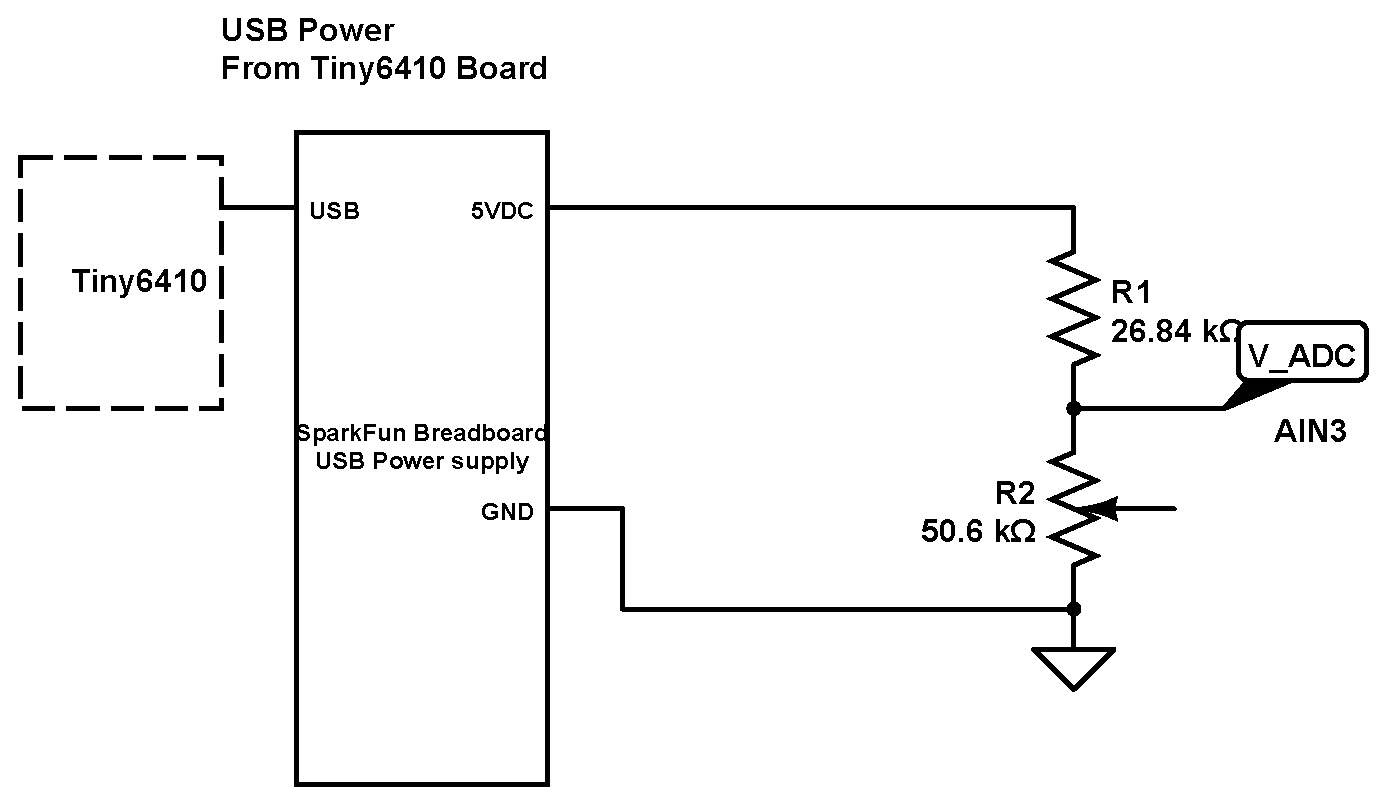
\includegraphics[scale=.35]{cmpe242_adc_validator}
	\caption{Schematic for Prototype Board}\label{cmpe242_adc_validator}
\end{figure}

\begin{figure}[ht!]
	\includegraphics[scale=.15]{cmpe242_lab2.jpg}
	\caption{Photo of the entire setup}\label{cmpe242_lab2_photo}
\end{figure}

A 5VDC power source was used to drive the ADC validation circuit. The measured maximum resistance of the potentiometer is $50.6k\Omega$. The maximum allowed voltage into the ADC is 3.3VDC. Therefore, referring to equation \ref{VoltageDivider}, the potentiometer is $R_2$ and the required resistance for $R_1$ is $26k\Omega$. The measured resistance is $26.84k\Omega$ using standard 5\% resistors.

\subsection{Software}
The user level program will acquire as many data points as requested by the user. Each data point is acquired from the ADC every ($\frac{1}{10}$) second. Once all of the data has been collected, the FFT is calculated for the data and the power spectrum is calculated. Furthermore, the data from the ADC as well as the FFT value for each data point is written out to a comma separated value (CSV) file for further review and analysis. 
A screenshot of the user level program in action can be found in \ref{lab2inaction}.

\begin{figure}[ht!]
	\includegraphics[scale=.55]{lab2inaction.jpg}
	\caption{Screen Shot of User Level Program}\label{lab2inaction}
\end{figure}


%
% Testing and Verification
%
\section{Testing and Verification}
\subsection{Fourier Analysis}
The data from the ADC was read several times in several different configurations,
\begin{enumerate}
	\item 256 and 1024 data points at 0VDC, \ref{power_spectrum_0_1024}
	\item 256 and 1024 data points at Various voltages from 0--3.3VDC, \ref{power_spectrum_0_33_1024}
	\item 256 and 1024 data points at 3.3VDC, \ref{power_spectrum_33_1024}
\end{enumerate}

The results from the FFT were very good as nearly all of the power was at the zero frequency, which is what to be expected for DC values.
\begin{figure}[ht]
	\includegraphics[scale=.50]{power_spectrum_0_1024}
	\caption{Power Spectrum for 0VDC and N = 1024}\label{power_spectrum_0_1024}
\end{figure}
\begin{figure}[ht]
	\includegraphics[scale=.50]{power_spectrum_0_33_1024}
	\caption{Power Spectrum for 0--3.3VDC and N = 1024}\label{power_spectrum_0_33_1024}
\end{figure}
\begin{figure}[ht]
	\includegraphics[scale=.50]{power_spectrum_33_1024}
	\caption{Power Spectrum for 33VDC and N = 1024}\label{power_spectrum_33_1024}
\end{figure}

The results from the linear test were nearly perfect. 15 data points were recorded and the data, along with a best fit line can be found in figure \ref{linear_data}.

\begin{figure}[ht]
	\includegraphics[scale=.50]{linear_data}
	\caption{Linear Relationship between Voltage and ADC}\label{linear_data}
\end{figure}

\pagebreak

%
% Conclusion
%
\section{Conclusion}
In conclusion, the ADC was shown to be working properly. Manually checking the voltage and the ADC valued revealed that the ADC operates linearly and in an expected fashion. The validation using the power spectrum and the Fast Fourier Transform shows a valid ADC for multiple bit resolutions and multiple data points.


%
% thebibliography
%
\begin{thebibliography}{9}
\bibitem{LDD}
Jonathan Corbet, Alessandro Rubini, and Greg Kroah-Hartman,
\emph{Linux Device Drivers, Third Edition},
O'Reilly Media,
Sebastopol, CA,
2005

\bibitem{Samsung}
-,
\emph{User's Manual \\ S3C6410X \\ RISC Microprocessor},
Samsung Electronics, Inc.,
2008

\bibitem{HWHandout}
Harry Li,
\emph{Handout On Hardware of the ARM11 Development Board},
Computer Engineering Department, College of Engineering,
 San Jose State University,
Spring, 2013

\bibitem{FFTHandout}
Harry Li,
\emph{Handout On The Fast Fourier Transform},
Computer Engineering Department, College of Engineering,
 San Jose State University,
Spring, 2013

\bibitem{USB5VDC}
- (31 Mar. 2013),
\emph{Breadboard Power Supply USB - 5V/3.3V.}
[Online]
Available: https://www.sparkfun.com/products/8376

\bibitem{ARMSales}
Agam Shah (Jan 22, 2013)
\emph{Processor market to get boost from smartphones, tablets}
[Online]
Available: http://www.pcworld.com/article/2025967/processor-market-to-get-boost-from-smartphones-tablets.html

\bibitem{FFTO}
- (March 23, 2013)
\emph{Fast Fourier transform}
[Online]
Available: https://en.wikipedia.org/wiki/Fast\_Fourier\_transform

\end{thebibliography}

\end{document}
